\pdfoutput=1
\documentclass[12pt]{article}
% Load preamble (packages, math, definitions, comments)
%\RequirePackage[l2tabu, orthodox]{nag}

% FONTS
\usepackage[utf8]{inputenc} % allow utf-8 input
\usepackage[T1]{fontenc}    % use 8-bit T1 fonts

% Replace default Latin Modern typewriter with its proportional counterpart
% http://www.tug.dk/FontCatalogue/lmoderntypewriterprop/
\renewcommand*\ttdefault{lmvtt}


%%% OPTION 1 - Fourier Math + New Century Schoolbook + ParaType Sans

% % Import Fourier Math (this imposes its own New Century Schoolbook type)
% % http://www.ctan.org/tex-archive/fonts/fouriernc/
% \usepackage{fouriernc}
% \usepackage{amsmath}
% % Replace with TeX Gyre Schola version of New Century Schoolbook (must scale!)
% % http://www.tug.dk/FontCatalogue/tgschola/
% \usepackage[scale=0.92]{tgschola}
% \usepackage[scaled=0.88]{PTSans}

%% OPTION 2 - MathDesign Math + Bitstream Charter + ParaType Sans

% Import MathDesign (this brings along Bitstream Charter)
% http://www.ctan.org/tex-archive/fonts/mathdesign/
\usepackage[bitstream-charter]{mathdesign}
\usepackage{amsmath}
\usepackage[scaled=0.92]{PTSans}


% %%% OPTION 3 - MTPRO 2 Math + Termes Times + ParaType Sans

% \usepackage{tgtermes}
% \usepackage{amsmath}
% \usepackage[subscriptcorrection,
%             amssymbols,
%             mtpbb,
%             mtpcal,
%             nofontinfo  % suppresses all warnings
%            ]{mtpro2}
% \usepackage{scalefnt,letltxmacro}
% \LetLtxMacro{\oldtextsc}{\textsc}
% \renewcommand{\textsc}[1]{\oldtextsc{\scalefont{1.10}#1}}
% \usepackage[scaled=0.92]{PTSans}

% GEOMETRY
\usepackage[
  paper  = letterpaper,
  left   = 1.0in,
  right  = 1.0in,
  top    = 1.0in,
  bottom = 1.0in,
  ]{geometry}

% COLOR
\usepackage[usenames,dvipsnames,table]{xcolor}
%\usepackage[usenames,table]{xcolor}
\definecolor{shadecolor}{gray}{0.9}

% SPACING and TEXT
\usepackage[final,expansion=alltext]{microtype}
\usepackage[english]{babel}
\usepackage[parfill]{parskip}
\usepackage{afterpage}
\usepackage{framed}

%redefine the leftbar environment to accept a width and coloring options
\renewenvironment{leftbar}[1][\hsize]
{%
  \def\FrameCommand
  {%
    {\color{Gray}\vrule width 3pt}%
    \hspace{10pt}%
    %\hspace{0pt}\fboxsep=\FrameSep\colorbox{black!10}%
  }%
  \MakeFramed{\hsize#1\advance\hsize-\width\FrameRestore}%
}%
{\endMakeFramed}

% define a paragraph header function
\DeclareRobustCommand{\parhead}[1]{\textbf{#1}~}

% EDITING
% line numbering in left margin
\usepackage{lineno}
\renewcommand\linenumberfont{\normalfont
                             \footnotesize
                             \sffamily
                             \color{SkyBlue}}
% ragged paragraphs in right margin
\usepackage{ragged2e}
\DeclareRobustCommand{\sidenote}[1]{\marginpar{
                                    \RaggedRight
                                    \textcolor{Plum}{\textsf{#1}}}}
% paragraph counter in right margin
\newcommand{\parnum}{\bfseries\P\arabic{parcount}}
\newcounter{parcount}
\newcommand\p{%
    \stepcounter{parcount}%
    \leavevmode\marginpar[\hfill\parnum]{\parnum}%
}
% paragraph helper
\DeclareRobustCommand{\PP}{\textcolor{Plum}{\P} }

% COUNTERS
\renewcommand{\labelenumi}{\color{black!67}{\arabic{enumi}.}}
\renewcommand{\labelenumii}{{\color{black!67}(\alph{enumii})}}
\renewcommand{\labelitemi}{{\color{black!67}\textbullet}}

% FIGURES
\usepackage{graphicx}
\usepackage{float}  % for the [H] float placement specifier
\usepackage{wrapfig}
\usepackage[labelfont=bf,font=footnotesize,width=.9\textwidth]{caption}
\usepackage[format=hang]{subcaption}

% TABLES
\usepackage{booktabs,multirow,multicol}       % professional-quality tables

% ALGORITHMS
\usepackage[algoruled]{algorithm2e}
\usepackage{listings}
\usepackage{fancyvrb}
\fvset{fontsize=\normalsize}

% BIBLIOGRAPHY
% Note: natbib is loaded in main.tex (after document class)
% For biblatex instead, use: \usepackage[%
minnames=1,maxnames=99,maxcitenames=2,
style=alphabetic,
doi=false,
url=false,
firstinits=true,
hyperref,
natbib,
backend=bibtex,
sorting=nyt
]{biblatex}%

\newbibmacro*{journal}{%
  \iffieldundef{journaltitle}
    {}
    {\printtext[journaltitle]{%
       \printfield[noformat]{journaltitle}%
       \setunit{\subtitlepunct}%
       \printfield[noformat]{journalsubtitle}}}}

\DeclareFieldFormat[article,inbook,incollection,inproceedings,patent,thesis,unpublished]{titlecase}{\MakeSentenceCase*{#1}}

\AtEveryBibitem{%
\ifentrytype{article}{
    \clearfield{url}%
    \clearfield{urldate}%
    \clearfield{eprint}
}{}
\ifentrytype{book}{
    \clearfield{url}%
    \clearfield{urldate}%
}{}
\ifentrytype{collection}{
    \clearfield{url}%
    \clearfield{urldate}%
}{}
\ifentrytype{incollection}{
    \clearfield{url}%
    \clearfield{urldate}%
}{}
}

\AtEveryBibitem{
    \clearfield{pages}
    \clearfield{review}%
    \clearfield{series}%%
    \clearfield{volume}
    \clearfield{pages}
    \clearfield{month}
    \clearfield{eprint}
    \clearfield{isbn}
    \clearfield{issn}
    \clearlist{location}
    \clearfield{series}
    \clearlist{publisher}
    \clearname{editor}
}{}

% HYPERREF
\usepackage[colorlinks,linktoc=all]{hyperref}
\usepackage[all]{hypcap}
\hypersetup{citecolor=MidnightBlue}
\hypersetup{linkcolor=MidnightBlue}
\hypersetup{urlcolor=MidnightBlue}

% CLEVEREF must come after HYPERREF
\usepackage[nameinlink,capitalise]{cleveref}
\Crefname{section}{\S}{\S}

% ACRONYMS
\usepackage[acronym,nowarn]{glossaries}
% Define an acronym style with small caps
\renewcommand*{\acronymfont}[1]{\textsc{#1}}

% COLOR DEFINITIONS
\newcommand{\red}[1]{\textcolor{BrickRed}{#1}}
\newcommand{\orange}[1]{\textcolor{BurntOrange}{#1}}
\newcommand{\green}[1]{\textcolor{OliveGreen}{#1}}
\newcommand{\blue}[1]{\textcolor{MidnightBlue}{#1}}
\newcommand{\gray}[1]{\textcolor{black!60}{#1}}

% LISTINGS DEFINTIONS
\lstdefinestyle{mystyle}{
    commentstyle=\color{OliveGreen},
    keywordstyle=\color{BurntOrange},
    numberstyle=\tiny\color{black!60},
    stringstyle=\color{MidnightBlue},
    basicstyle=\ttfamily,
    breakatwhitespace=false,
    breaklines=true,
    captionpos=b,
    keepspaces=true,
    numbers=left,
    numbersep=5pt,
    showspaces=false,
    showstringspaces=false,
    showtabs=false,
    tabsize=2
}
\lstset{style=mystyle}

% MATH PACKAGES AND DEFINITIONS
% !TEX root = main.tex

% MATH PACKAGES
% Note: amsfonts conflicts with mathdesign (loaded in preamble.tex)
% mathdesign provides its own blackboard bold, so we skip amsfonts
\usepackage{centernot}
\usepackage{amsthm}         % theorem environments
\usepackage{nicefrac}       % compact symbols for 1/2, etc.
\usepackage{mathtools}      % extends amsmath
\usepackage{amsbsy}         % bold math symbols
\usepackage{amstext}        % text in math mode
\usepackage{thmtools}       % theorem tools
\usepackage{thm-restate}    % restatable theorems

% compatibility w/ parskip https://tex.stackexchange.com/questions/25346/wrong-spacing-before-theorem-environment-amsthm
\begingroup
    \makeatletter
    \@for\theoremstyle:=definition,remark,plain\do{%
        \expandafter\g@addto@macro\csname th@\theoremstyle\endcsname{%
            \addtolength\thm@preskip\parskip
            }%
        }
\endgroup

\DeclareRobustCommand{\mb}[1]{\ensuremath{\mathbf{\boldsymbol{#1}}}}
% \DeclareRobustCommand{\mb}[1]{\mathbold{#1}}

\DeclareRobustCommand{\KL}[2]{\ensuremath{\textrm{KL}\left(#1\;\|\;#2\right)}}

% \DeclareMathOperator*{\argmax}{arg\,max}
% \DeclareMathOperator*{\argmin}{arg\,min}

\crefname{lemma}{lemma}{lemmas}
\Crefname{lemma}{Lemma}{Lemmas}
\crefname{thm}{theorem}{theorems}
\Crefname{thm}{Theorem}{Theorems}
\crefname{prop}{proposition}{propositions}
\Crefname{prop}{Proposition}{Propositions}
\crefname{assumption}{assumption}{assumptions}
\crefname{assumption}{Assumption}{Assumptions}


% \newtheorem{thm}{Theorem} % reset theorem numbering for each chapter
% \newtheorem{defn}{Definition} % definition numbers are dependent on theorem numbers
% \newtheorem{prop}[thm]{Proposition}
% \newtheorem{exmp}[thm]{Example} % same for example numbers
% \newtheorem{lemma}[thm]{Lemma}
% \newtheorem{assumption}{Assumption}
% \newtheorem{corollary}[thm]{Corollary}
% Independence symbol (double perp): use \indpt
\def\independenT#1#2{\mathrel{\rlap{$#1#2$}\mkern2mu{#1#2}}}



\def\checkmark{\tikz\fill[scale=0.4](0,.35) -- (.25,0) -- (1,.7) -- (.25,.15) -- cycle;} 

% Note: booktabs loaded in preamble.tex; arydshln adds dashed lines
\usepackage{arydshln}
\makeatletter
\def\adl@drawiv#1#2#3{%
        \hskip.5\tabcolsep
        \xleaders#3{#2.5\@tempdimb #1{1}#2.5\@tempdimb}%
                #2\z@ plus1fil minus1fil\relax
        \hskip.5\tabcolsep}
\newcommand{\cdashlinelr}[1]{%
  \noalign{\vskip\aboverulesep
           \global\let\@dashdrawstore\adl@draw
           \global\let\adl@draw\adl@drawiv}
  \cdashline{#1}
  \noalign{\global\let\adl@draw\@dashdrawstore
           \vskip\belowrulesep}}
\makeatother

\newenvironment{proofsk}{%
  \renewcommand{\proofname}{Proof sketch}\proof}{\endproof}

\renewcommand{\epsilon}{\varepsilon}

%********************************************************************
% Extra theorem environments
%********************************************************************

\declaretheorem[style=plain,numberwithin=section,name=Theorem]{theorem}
\declaretheorem[style=plain,sibling=theorem,name=Lemma]{lemma}
\declaretheorem[style=plain,sibling=theorem,name=Proposition]{proposition}
\declaretheorem[style=plain,sibling=theorem,name=Corollary]{cor}
\declaretheorem[style=plain,sibling=theorem,name=Claim]{claim}
\declaretheorem[style=plain,sibling=theorem,name=Conjecture]{conj}
\declaretheorem[style=definition,sibling=theorem,name=Definition]{defn}
\declaretheorem[style=definition,name=Assumption]{assumption}
\declaretheorem[style=definition,sibling=theorem,name=Example]{example}
\declaretheorem[style=remark,sibling=theorem,name=Remark]{remark}

\newenvironment{example*}
 {\pushQED{\qed}\example}
 {\popQED\endexample}
\numberwithin{equation}{section}

% This file contains definitions of custom macros
% ------------------------------------------------------------------------------

\newcommand{\grad}{\nabla}
\newcommand\dif{\mathop{}\!\mathrm{d}}
\newcommand{\diag}{\textrm{diag}}
\newcommand{\supp}{\textrm{supp}}
\newcommand{\E}[2]{\mathbb{E}_{#1}\left[#2\right]}
\newcommand{\G}[2]{\mathbb{G}_{#1}\left[#2\right]}
\newcommand{\V}[2]{\mathbb{V}_{#1}\left[#2\right]}

\newcommand{\defeq}{\overset{\mathrm{def}}{=}}
\newcommand{\equalas}{\overset{\mathrm{a.s.}}{=}}
\newcommand{\disteq}{\overset{d}{=}}
\newcommand{\iidsim}{\overset{\mathrm{iid}}{\sim}}
\newcommand{\indsim}{\overset{\mathrm{ind}}{\sim}}

\newcommand{\Reals}{\mathbb{R}}
\newcommand{\Nats}{\mathbb{N}}
\newcommand{\NNReals}{\Reals_{+}}

\newcommand{\exclude}{\backslash}

\newcommand{\eps}{\varepsilon}

\DeclareMathOperator*{\argmin}{argmin}
\DeclareMathOperator*{\argmax}{argmax}
\DeclareMathOperator*{\logit}{logit}

\newcommand{\abs}[1]{\left\lvert#1 \right\rvert}

%%% Local Variables:
%%% mode: latex
%%% TeX-master: "main"
%%% End:


% DRAFT COMMENTS (switch to nocommenting for production)
%%%%%%%%%%%%%%%%%%%%%%%%%%%%%%%%%%%%%%%%%%%%%%%%%%%%%%%%%%
%%%% EDITING HELPER FUNCTIONS  %%%%%%%%%%%%%%%%%%%%%%%%%%%
%%%%%%%%%%%%%%%%%%%%%%%%%%%%%%%%%%%%%%%%%%%%%%%%%%%%%%%%%%

%% NA: needs attention (rough writing whose correctness needs to be verified)
%% TBD: instructions for how to fix a gap ("Describe the propagation by ...")
%% PROBLEM: bug or missing crucial bit 

%% use \fXXX versions of these macros to put additional explanation into a footnote.  
%% The idea is that we don't want to interrupt the flow of the paper or make it 
%% impossible to read because there are a bunch of comments.

%% NA's (and TBDs, those less crucially) should be written so 
%% that they flow with the text.

\definecolor{WowColor}{rgb}{.75,0,.75}
\definecolor{SubtleColor}{rgb}{0,0,.50}

% inline
\newcommand{\NA}[1]{\textcolor{SubtleColor}{ {\tiny \bf ($\star$)} #1}}
\newcommand{\LATER}[1]{\textcolor{SubtleColor}{ {\tiny \bf ($\dagger$)} #1}}
\newcommand{\TBD}[1]{\textcolor{SubtleColor}{ {\tiny \bf (!)} #1}}
\newcommand{\PROBLEM}[1]{\textcolor{WowColor}{ {\bf (!!)} {\bf #1}}}

% as margin notes

\newcounter{margincounter}
\newcommand{\displaycounter}{{\arabic{margincounter}}}
\newcommand{\incdisplaycounter}{{\stepcounter{margincounter}\arabic{margincounter}}}

\newcommand{\fTBD}[1]{\textcolor{SubtleColor}{$\,^{(\incdisplaycounter)}$}\marginpar{\raggedright\tiny\textcolor{SubtleColor}{ {\tiny $(\displaycounter)$} #1}}}

\newcommand{\fPROBLEM}[1]{\textcolor{WowColor}{$\,^{((\incdisplaycounter))}$}\marginpar{\raggedright\tiny\textcolor{WowColor}{ {\bf $\mathbf{((\displaycounter))}$} {\bf #1}}}}

\newcommand{\fLATER}[1]{\textcolor{SubtleColor}{$\,^{(\incdisplaycounter\dagger)}$}\marginpar{\raggedright\tiny\textcolor{SubtleColor}{ {\tiny $(\displaycounter\dagger)$} #1}}}

% % Production mode: error on leftover draft comments
% Switch to commenting.tex during drafting

\newcommand{\LATER}[1]{\PackageError{nocommenting}{Leftover LATER comment}{Remove all LATER comments before final build}}
\newcommand{\fLATER}[1]{\PackageError{nocommenting}{Leftover fLATER comment}{Remove all fLATER comments before final build}}
\newcommand{\TBD}[1]{\PackageError{nocommenting}{Leftover TBD comment}{Remove all TBD comments before final build}}
\newcommand{\fTBD}[1]{\PackageError{nocommenting}{Leftover fTBD comment}{Remove all fTBD comments before final build}}
\newcommand{\PROBLEM}[1]{\PackageError{nocommenting}{Leftover PROBLEM comment}{Remove all PROBLEM comments before final build}}
\newcommand{\fPROBLEM}[1]{\PackageError{nocommenting}{Leftover fPROBLEM comment}{Remove all fPROBLEM comments before final build}}
\newcommand{\NA}[1]{#1}


% Bibliography: natbib (for biblatex, see preamble/minimalist_biblatex.tex)
\usepackage{natbib}
% Provides author/affiliation formatting with italic affiliations
\usepackage[affil-it]{authblk}

\title{TNBBeta-VAE Research Summary: Week 1}
% \date{}
\author[1]{Vedant Pathak}

\affil[1]{Department of Statistics, University of Chicago}
\date{September 26\textsuperscript{th}, 2026}

\begin{document}
\maketitle

\section{Overview}
The goal of this week's research was to produce a working VAE using the spherical
TNBBeta distribution as a variational approximation to the true posterior
on at least one dataset. By ``working,'' I simply mean stable convergence of the
-ELBO objective. I was able to get that out of the way on day 1 and spent the rest
of the week replicating the experiments in \citep{davidson2022hypersphericalvariationalautoencoders}
and understanding where this spherical approach sits relative to the existing
vMF-based (S-VAE) approach.

On all experiments I ran, both spherical VAEs' results matched. What is even more
curious is that the geometry of the TNBBeta-VAE's latent space appears to match
that of the S-VAE. The additional expressivity gained from the TNBBeta is thrown
away during training, and the per-point posteriors converge to caps on the unit
hypersphere.

\section{Recap and Problem Setup}
Recall the definition of the triply-randomized negative binomial beta (TNBBeta)
distribution introduced in \citep{lederman2026triplyrandomizednegativebinomialbeta}:
\begin{align*}
    \text{TNBBeta}(y; p, q, \varepsilon) &= \text{beta}(y; \varepsilon, \varepsilon)\left[\frac{1 - q}{y(1 - y)}\gamma(y, p)\right]^{\varepsilon}\left[1 - 4q\gamma(y, p)\right]^{-\left(\varepsilon + \frac{1}{2}\right)} \\
    \gamma(y, p) &\defeq \frac{1}{4}\text{sech}^2\left(\frac{\text{logit}(y) - \text{logit}(p)}{2}\right)
\end{align*}
In the above distribution supported on $[0, 1]$, $p$ governs the median, $q$
governs the concentration about $p$, and $\varepsilon$ governs tail behavior.
Notably, one can obtain a TNBBeta sample via a deterministic transformation of
a beta-distributed sample, as is outlined in \Cref{alg:tnbbeta-sample} in the construction of $Y$.
One may then apply a householder reflection to lift $Y$ to the unit sphere.
\begin{algorithm}[H]
    \caption{Sampling $\mathbf{z} \sim \mathrm{SphericalTNBBeta}(\boldsymbol{\mu}, p, q, \varepsilon)$}
    \label{alg:tnbbeta-sample}
    \KwIn{Mean direction $\boldsymbol{\mu} \in S^{d-1}$, median $p \in (0, 1)$, concentration
        $q \in [0, 1)$, boundary parameter $\varepsilon > 0$.}
    \KwOut{$\mathbf{z} \sim \mathrm{SphericalTNBBeta}(\boldsymbol{\mu}, p, q, \varepsilon)$.}
    Draw $Z \sim \mathrm{Beta}(\varepsilon, \varepsilon)$ \\
    $S \leftarrow 2Z - 1$ \\
    $U \leftarrow \dfrac{1}{2}\left(1 + S\sqrt{\dfrac{1 - q}{1 - qS^2}}\right)$ \\
    $Y \leftarrow \dfrac{pU}{(1 - p)(1 - U) + pU}$ \\
    $W \leftarrow 2Y - 1$ \\
    Draw $\mathbf{g} \sim \mathcal{N}(\mathbf{0}, I_{d-1})$, $\mathbf{v} \leftarrow \mathbf{g} / \|\mathbf{g}\|$ \\
    $\mathbf{x} \leftarrow \left(W, \sqrt{1 - W^2}\,\mathbf{v}\right)$ \\
    \eIf{$\boldsymbol{\mu} = \mathbf{e}_1$}{
        $\mathbf{z} \leftarrow \mathbf{x}$
    }{
        $\mathbf{d} \leftarrow \mathbf{e}_1 - \boldsymbol{\mu}$ \\
        $\mathbf{u} \leftarrow \mathbf{d} / \|\mathbf{d}\|$ \\
        $\mathbf{z} \leftarrow \mathbf{x} - 2(\mathbf{u}^\top \mathbf{x})\mathbf{u}$
    }
    \Return{$\mathbf{z}$}
\end{algorithm}
Let the distribution of the resulting random unit vector $\mathbf{z}$ be defined
as SphericalTNBBeta, the density of which is given by
\[
    \text{SphericalTNBBeta}(\mathbf{z}; \boldsymbol{\mu}, p, q, \varepsilon) = \frac{1}{2}\text{TNBBeta}(y; p, q, \varepsilon)\left(1 - w^2\right)^{-\frac{d - 3}{2}}\left|\mathcal{S}^{d - 2}\right|^{-1}
\]
where $w, y$ are realizations of $W, Y$ as outlined in \Cref{alg:tnbbeta-sample}.

\cref{fig:pq-ablation} illustrates the TNBBeta distribution as well as its corresponding
spherical distribution for $\boldsymbol{\mu} = \mathbf{e}_3$. Most notably, note that
for $p = 0.95, q = 0, \varepsilon=1$, one observes a similar density to the vMF for a
given concentration $\kappa$. That aside, the SphericalTNBBeta clearly admits greater
expressivity. For future reference, it is simply worth noting that one may obtain a
``cap''-like and a ``ring''-like density as illustrated above.

Given that one may sample a SphericalTNBBeta random variable from noise, one could leverage
the SphericalTNBBeta as the variational approximation to the posterior on a hyperspherical
latent space VAE. It follows that this choice of posterior obeys the reparametrization trick
enabling low-variance gradient estimation. To understand the implications of such a choice,
I ran the same experiments as \citep{davidson2022hypersphericalvariationalautoencoders} with
some additions of my own to understand how the TNBBeta-VAE differs from the S-VAE proposed by
the authors.

\begin{figure}[H]
    \centering
    \begin{subfigure}[t]{0.49\textwidth}
        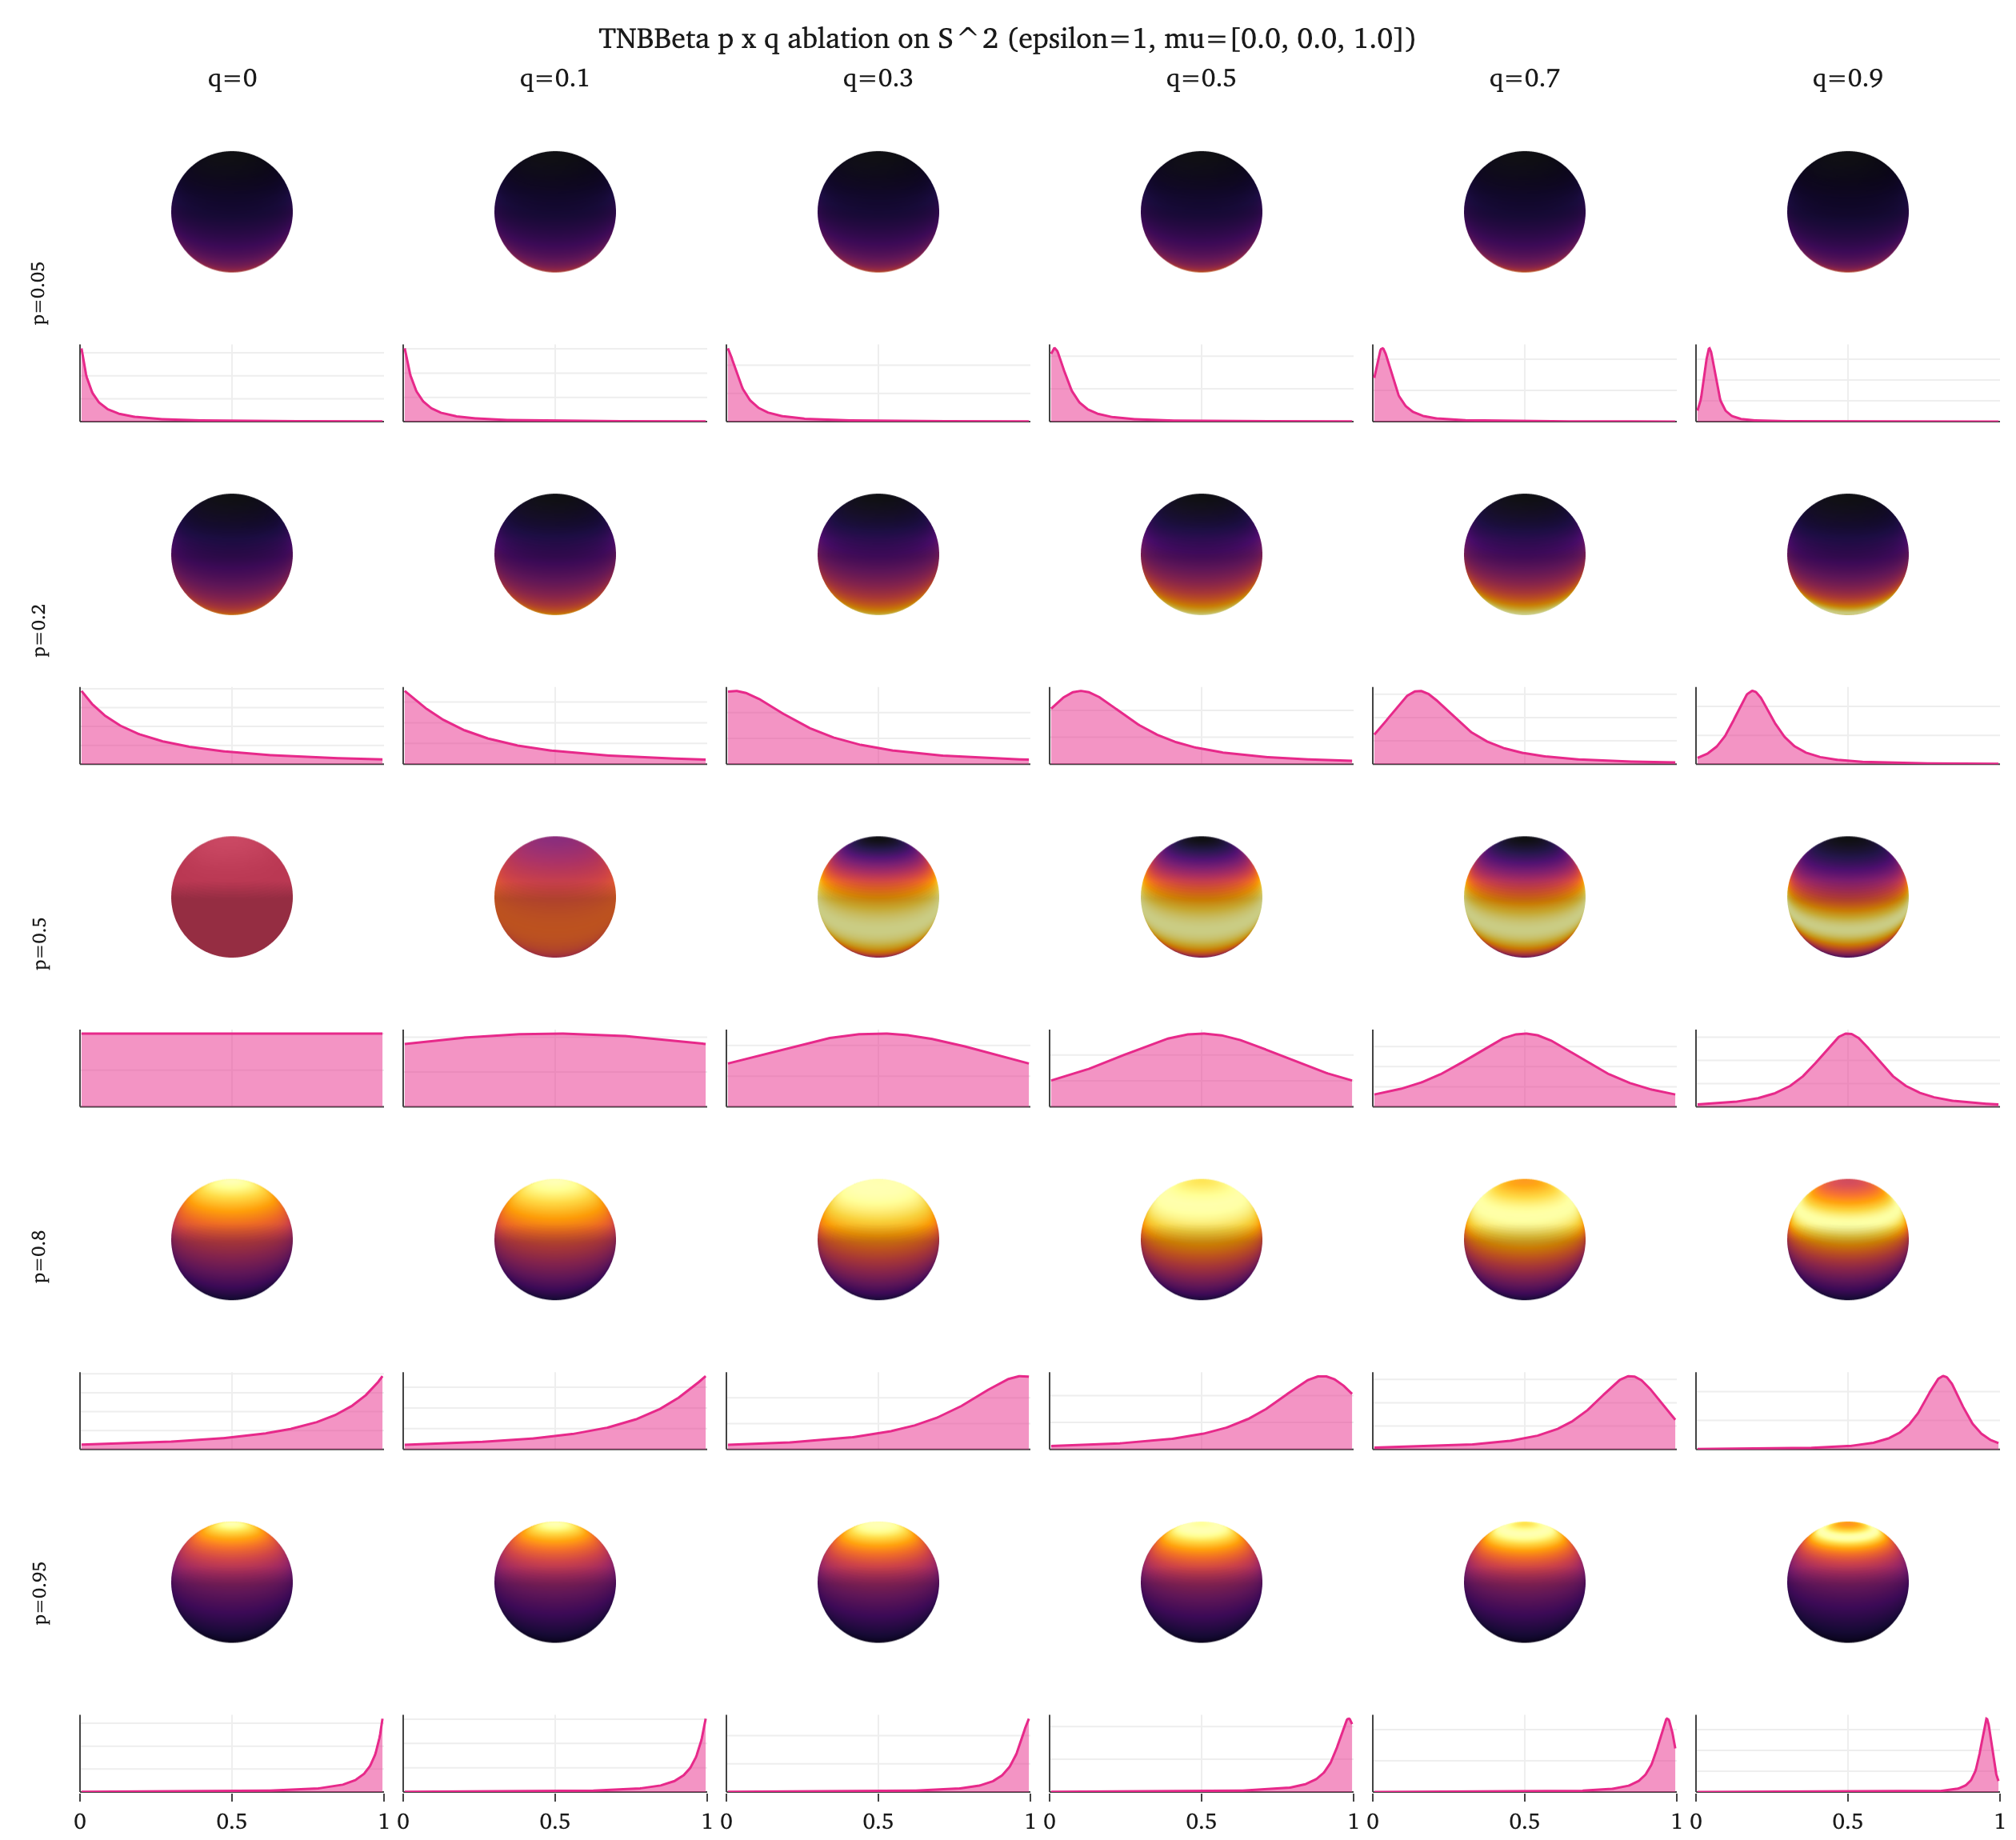
\includegraphics[width=\linewidth]{assets/pq_ablation.png}
        \caption{$p \times q$ ablation ($\varepsilon = 1$).}
        \label{fig:pq-ablation}
    \end{subfigure}
    \hfill
    \begin{subfigure}[t]{0.49\textwidth}
        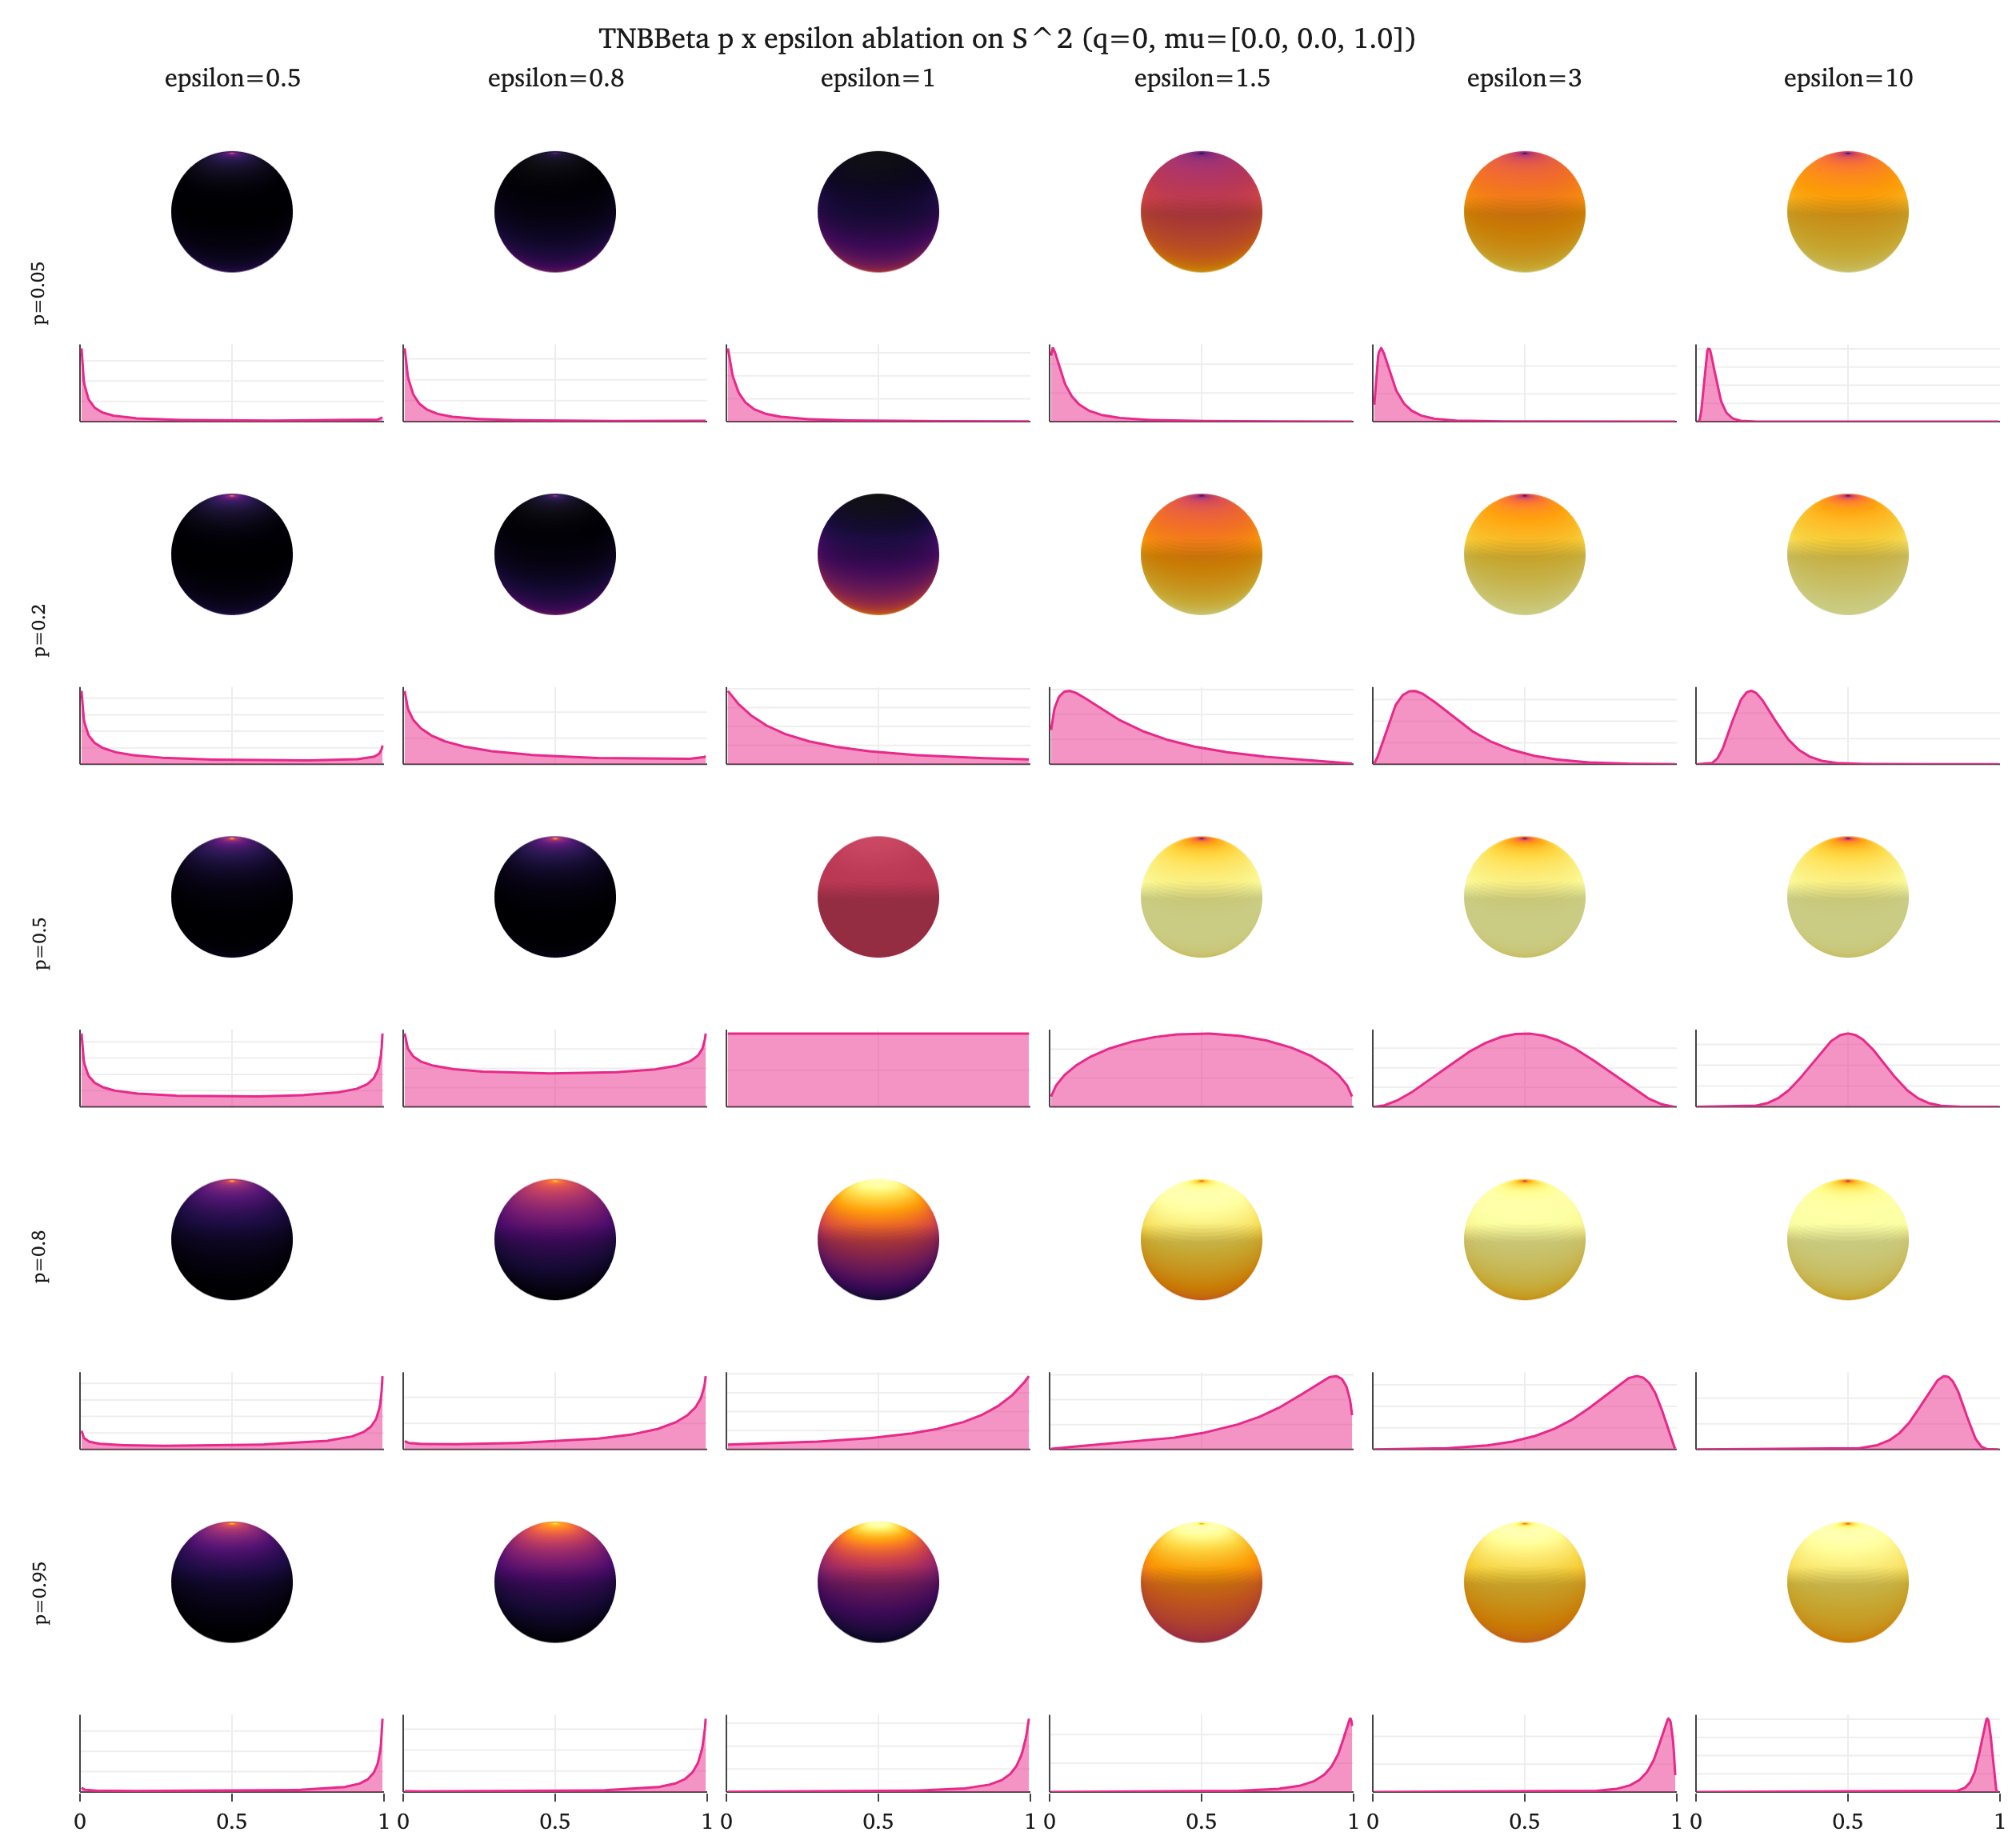
\includegraphics[width=\linewidth]{assets/p_epsilon_ablation.png}
        \caption{$p \times \varepsilon$ ablation ($q = 0$).}
        \label{fig:p-epsilon-ablation}
    \end{subfigure}
    \caption{TNBBetaSpherical on $S^2$ ($\mu = [0, 0, 1]$): each cell shows the
    spherical log-density above its corresponding univariate density on $(0, 1)$.}
    \label{fig:ablations}
\end{figure}


\section{Results}
\label{sec:results}
\citep{davidson2022hypersphericalvariationalautoencoders} propose an algorithm to sample
a $\text{vMF}(\mathbf{\boldsymbol{\mu}}, \kappa)$ random variable that relies on rejection sampling.
This has obvious speed limitations and as such I sought out to understand how much faster
it is to sample a SphericalTNBBeta random variable on a single GPU. \Cref{fig:speed-heatmap}
shows that SphericalTNBBeta sampling is at least twice as fast as vMF sampling, and
depending on the latent dimension, batch size, and concentration parameter, this ratio
dramatically increases.
\begin{figure}[H]
    \centering
    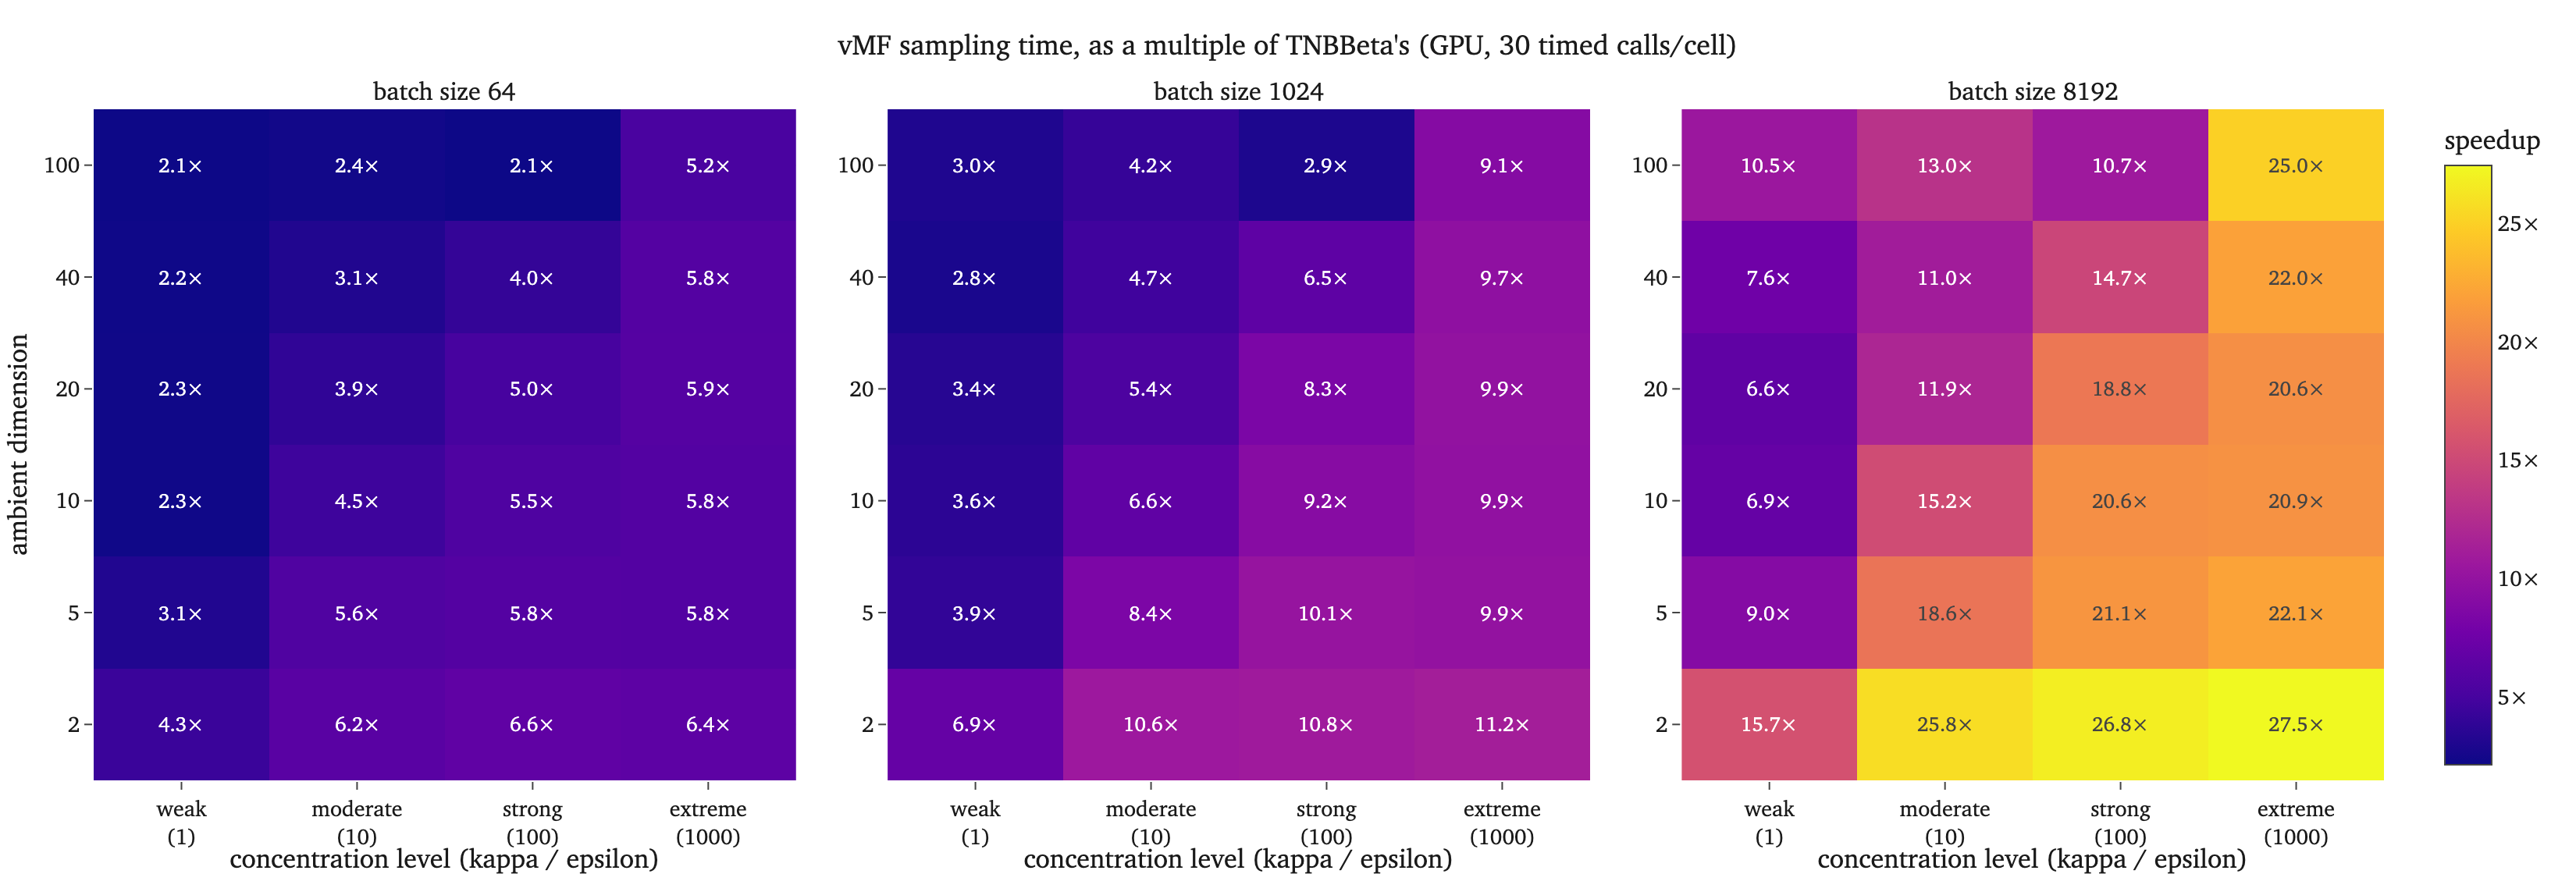
\includegraphics[width=\linewidth]{assets/sampling_speed_heatmap.png}
    \caption{Comparison of sampling runtime between SphericalTNBBeta and vMF distributions.}
    \label{fig:speed-heatmap}
\end{figure}
To understand where the TNBBeta sits in relation to the vMF and Gaussian VAEs, I replicated
table 1 from \citep{davidson2022hypersphericalvariationalautoencoders}, this time adding the
TNBBeta-VAE's results. Namely, I trained a series of VAEs on binarized MNIST using a
convolutional\footnote{Implementation details can be found here: https://github.com/Dant86/tnbbeta\_vae}
encoder and decoder. \Cref{tab:mnist-table1} outlines performance on the test set over varying
latent dimensions. Note that $d$ denotes the manifold dimension in line with the reference
paper's methodology. In particular, a spherical embedding for $d=2$ lies in $\mathbb{S}^2 \subset \mathbb{R}^3$.

\begin{table}[H]
    \centering
    \resizebox{\textwidth}{!}{%
    \begin{tabular}{lcccccccccccc}
        \toprule
        & \multicolumn{4}{c}{N-VAE} & \multicolumn{4}{c}{vMF} & \multicolumn{4}{c}{SphericalTNBBeta} \\
        \cmidrule(lr){2-5} \cmidrule(lr){6-9} \cmidrule(lr){10-13}
        $d$ & LL & $\mathcal{L}[q]$ & RE & KL & LL & $\mathcal{L}[q]$ & RE & KL & LL & $\mathcal{L}[q]$ & RE & KL \\
        \midrule
        2  & $-132.64_{\pm 0.30}$ & $-136.81_{\pm 0.28}$ & $-129.19_{\pm 0.35}$ & $7.62_{\pm 0.10}$ & $-130.86_{\pm 0.43}$ & $-134.42_{\pm 0.42}$ & $-126.89_{\pm 0.47}$ & $7.53_{\pm 0.08}$ & $-130.11_{\pm 0.57}$ & $-134.21_{\pm 0.46}$ & $-126.43_{\pm 0.54}$ & $7.78_{\pm 0.11}$ \\
        5  & $-105.38_{\pm 0.11}$ & $-109.53_{\pm 0.09}$ & $-96.12_{\pm 0.12}$ & $13.41_{\pm 0.17}$ & $-105.27_{\pm 0.14}$ & $-109.32_{\pm 0.08}$ & $-95.56_{\pm 0.12}$ & $13.76_{\pm 0.06}$ & $-104.89_{\pm 0.22}$ & $-109.15_{\pm 0.22}$ & $-95.36_{\pm 0.26}$ & $13.79_{\pm 0.13}$ \\
        10 & $\mathbf{-88.75_{\pm 0.12}}$ & $\mathbf{-92.91_{\pm 0.14}}$ & $-72.38_{\pm 0.10}$ & $20.53_{\pm 0.12}$ & $-89.38_{\pm 0.02}$ & $-93.60_{\pm 0.06}$ & $-71.84_{\pm 0.08}$ & $21.77_{\pm 0.05}$ & $-89.29_{\pm 0.10}$ & $-93.65_{\pm 0.14}$ & $-71.96_{\pm 0.25}$ & $21.69_{\pm 0.14}$ \\
        20 & $\mathbf{-83.67_{\pm 0.09}}$ & $\mathbf{-87.64_{\pm 0.11}}$ & $-61.87_{\pm 0.14}$ & $25.77_{\pm 0.07}$ & $-86.84_{\pm 0.04}$ & $-92.10_{\pm 0.05}$ & $-62.63_{\pm 0.21}$ & $29.47_{\pm 0.18}$ & $-86.90_{\pm 0.23}$ & $-92.12_{\pm 0.15}$ & $-62.33_{\pm 0.41}$ & $29.78_{\pm 0.53}$ \\
        40 & $-83.24_{\pm 0.05}$ & $-87.40_{\pm 0.07}$ & $-60.77_{\pm 0.11}$ & $26.63_{\pm 0.14}$ & $-144.28_{\pm 31.06}$ & $-170.06_{\pm 41.29}$ & $-162.32_{\pm 56.08}$ & $7.73_{\pm 14.79}$ & $-89.09_{\pm 0.15}$ & $-96.38_{\pm 0.14}$ & $-62.53_{\pm 0.42}$ & $33.86_{\pm 0.36}$ \\
        \bottomrule
    \end{tabular}%
    }
    \caption{Reproduction on binarized MNIST (conv encoder/decoder, 500-sample
        importance-weighted test log-likelihood, 5 seeds). N-VAE is the Gaussian baseline.
        $\mathcal{L}[q]$ is the ELBO, RE the reconstruction term, KL the exact KL
        (Gaussian, vMF) or a Monte Carlo estimate (TNBBeta, no closed form). \textbf{Bold}
        = best mean in the row, significant at $p < 0.01$ (Welch's $t$-test).}
    \label{tab:mnist-table1}
\end{table}
We see that for low dimensions, the vMF and SphericalTNBBeta VAEs perform similarly both in terms
of reconstruction error and KL. The vMF VAE becomes unstable in higher dimensions ($d=40$) and as such its
performance degrades, and while Gaussian is the clear winner, there's no sharp drop in performance for the
TNBBeta-VAE.

The fact that the S-VAE and TNBBeta-VAE perform similarly in low dimensions begs the question:
are the respective latent posteriors similar? A quick glance at the latent embeddings in the style
of \citep{davidson2022hypersphericalvariationalautoencoders} could give some signal:
\begin{figure}[H]
    \centering
    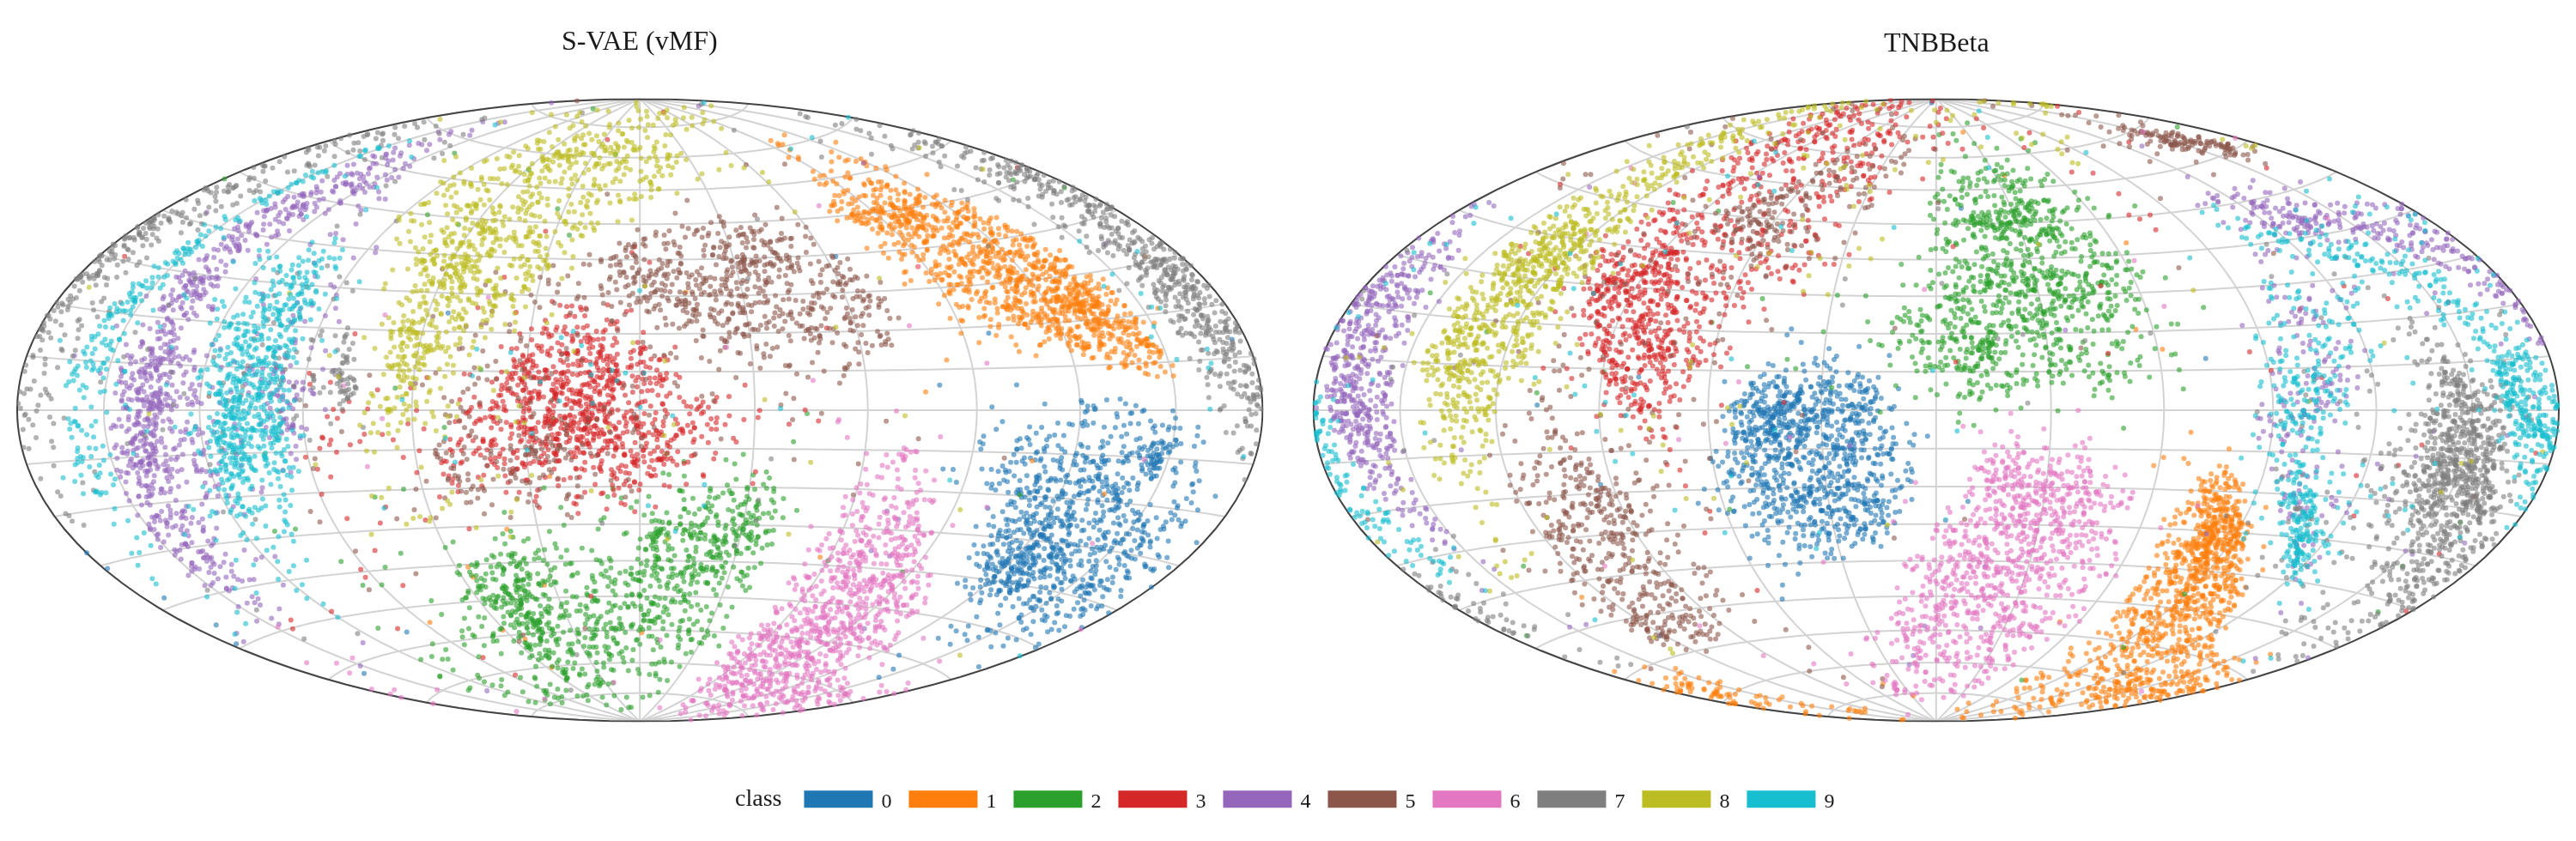
\includegraphics[width=\textwidth]{assets/hammer_mnist_vmfs_d2_seed0_vs_mnist_tnbs_d2_seed0.png}
    \caption{Hammer projection of latent embeddings in the S-VAE and TNBBeta-VAE trained on MNIST with $d=2$.}
    \label{fig:hammer}
\end{figure}
One very striking observation from the above is that both VAEs arrange MNIST class embeddings within
cap-like clusters on the unit hypersphere. Based on the distribution heatmaps from \Cref{fig:ablations}
I found the observation for the TNBBeta-VAE quite striking: the heatmaps show that, depending on the
parameters $p, q, \varepsilon$, mass is often concentrated about a ring on the unit hypersphere
as opposed to a cap. While running these experiments I often noticed that the SphericalTNBBeta posterior
would often converge to $p \to 1, q \to 0$ (see the bottom-left corner
of \Cref{fig:pq-ablation}) which does in fact concentrate mass about a cap, and not a ring. To verify this in higher dimensions,
I attempted to quantify ``ring-ness''. Claude Sonnet 5 suggested running an experiment to determine whether any mass
per MNIST class was distributed about a ring at all. 

\Cref{tab:ring-exclusion} includes the first diagnostic I used to determine whether any MNIST classes'
embeddings were distributed about a cap on the unit hypersphere. The "far-side \%" metric is computed
as follows: for each MNIST class, we compute the centroid embedding, and calculate the percent of
embeddings across the test set within that class that have negative cosine similarity to the
centroid. The ``antipodal \%" metric is calculated similarly, but we instead calculate the percent of
embeddings that have cosine similarity less than -0.9. This percentage is then averaged across all classes
for both metrics.
\begin{table}[H]
\centering
\begin{tabular}{lcccc}
\toprule
& \multicolumn{2}{c}{Far-side (\%)} & \multicolumn{2}{c}{Antipodal (\%)} \\
\cmidrule(lr){2-3} \cmidrule(lr){4-5}
$d$ & S-VAE (vMF) & TNBBeta & S-VAE (vMF) & TNBBeta \\
\midrule
2  & 1.56 $\pm$ 0.29 & 2.16 $\pm$ 0.71 & 0.12 $\pm$ 0.02 & 0.12 $\pm$ 0.05 \\
5  & 0.39 $\pm$ 0.04 & 0.37 $\pm$ 0.04 & 0.00 $\pm$ 0.00 & 0.00 $\pm$ 0.00 \\
10 & 0.52 $\pm$ 0.05 & 0.52 $\pm$ 0.04 & 0.00 $\pm$ 0.00 & 0.00 $\pm$ 0.00 \\
20 & 1.77 $\pm$ 0.11 & 1.77 $\pm$ 0.10 & 0.00 $\pm$ 0.00 & 0.00 $\pm$ 0.00 \\
40 & 3.00 $\pm$ 0.14 & 2.83 $\pm$ 0.06 & 0.00 $\pm$ 0.00 & 0.00 $\pm$ 0.00 \\
\bottomrule
\end{tabular}
\caption{Ring-shape check: percentage of each class's points more than
$90^\circ$ (respectively, within $0.9$ cosine of the exact antipode) from their own
class's centroid direction. Mean $\pm$ std over 5 seeds.}
\label{tab:ring-exclusion}
\end{table}
If the mass of each class-conditional distribution is, in fact, concentrated about a cap, then
one expects both metrics above to be extremely low: all embeddings should align closely with
the centroid. If ``far-side \%'' is high and ``antipodal \%'' is low, then we have reason to
believe that the class embeddings form a ring-like distribution. Based on the above results, though,
there is no evidence to believe that such a ring-like structure is ever taken on.

\section{Open Questions}
It's surprising that, despite all the expressivity of the univariate TNBBeta distribution,
there is little difference between the latent spaces in both hyperspherical VAEs tested above.
It would be worth understanding whether this is a theoretical necessity, or if this is simply
a domain-specific quirk that may not hold in other datasets. I tried fixing some parameters
to see if I could force ring-like posteriors. Fixing $\boldsymbol{\mu}$ only resulted in
situations in which $p \to 0$ and $q \to 1$. When I fixed $\varepsilon$, $q$ replaced $\varepsilon$
as a concentratio parameter in the posterior. Essentially, I have a sense that the S-VAE and
TNBBeta-VAE are producing highly similar posteriors in low dimensions, and I would like to understand
why.

Additionally, the SphericalTNBBeta VAE presents an alternative to the S-VAE that has faster sampling
and is more stable in high dimensions. This is the same conclusion as \citep{decao2020powersphericaldistribution}'s
power spherical distribution. In this light, it is worth understanding how these two hyperspherical
approaches to VAEs differ.

\section*{Acknowledgement of Generative AI Use}
Generative AI (specifically, Claude Sonnet 5) was used in the generation of all code to assist
with running the above experiments, as well as generating the above visualizations. I assert
that I have reviewed the above results and claim responsibility for the above statements. All
commentary in the writeup aside from the captions is my own. So is all analysis above.

\bibliographystyle{plainnat}
\bibliography{references}

\end{document}
